\section{Discussion}

\subsection{The non-homogeneous case}
If one were to solve the Poisson problem with non-homogeneous boundary conditions ie. $u = g(x) $ on $\partial \Omega$, 
some minor modifications would have to be done. 
The matrix system that is generated through this algorithm does not include the effect of the boundary elements, 
and in practice this is the same as assuming that they are equal zero. The second order differential operator on the elements 
closest to the boundary are on the form 
\begin{equation}
	-\frac{\partial^2 u_{i,j}}{\partial x^2} = -\frac{u_{i-1,j}-2u_{i,j}}{h^2}
\end{equation}
The incrementations of $i,j$ will depend on which boundary the element is close to, but the form of the operator is nevertheless the same.
The effect on equation~\ref{eq:Matrix} is that the boundary element is added to the left side.
In the homogeneous case this does not affect the numerical algorithm, but in the non-homogeneous case the boundary value needs to be added to the 
right hand side as well. This is implemented before the FST is done and does not have any impact on the parallel implementation. 

\subsection{Variations in the loading function $f$}
The loading function simply needs to be evaluated in all the grid points and multiplied by the steplength, before the 
FST-procedure starts. The only thing that will differ from the serial code is the displacement each MPI process have.
In Figure~\ref{fig:f} three solutions to the poisson problem have been plotted, all with different loading functions. 

\subsection{Variations in the domain $\Omega$}
By defining the domain $\Omega = (0,L_x)\times(0,L_y)$ but keeping the same number of grid points in each direction 
the discretization of the laplacian operator would be changed. In the unit square the discrete laplacian is defined as 
\begin{equation}
	\Delta u_{i,j} = \frac{u_{i-1,j}-2u_{i,j}+u_{i+1,j}}{h^2}+\frac{u_{i,j-1}-2u_{i,j}+u_{i,j+1}}{h^2}.
\end{equation}
In the new domain the operator would be defined as  
\begin{equation}
	\Delta u_{i,j} = \frac{u_{i-1,j}-2u_{i,j}+u_{i+1,j}}{h_x^2}+\frac{u_{i,j-1}-2u_{i,j}+u_{i,j+1}}{h_y^2}.
\end{equation}
Where $h_x=L_x/n$ and $h_y=L_y/n$ defines the new steplengths in each direction. Notice that the infamous 5-point formula now takes quite a 
different form and some rewriting is necessary. 
The diagonalized matrix system will now end up looking as 
\begin{equation}
	\left( \frac{1}{h_x^2}\underline{T} \; \underline{U}+\frac{1}{h_y^2}\underline{U}\; \underline{T} \right) _{i,j}=f_{i,j}
\end{equation}
By continuing the diagonalization procedure st. $\underline{T}=\underline{Q}\;\underline{\Lambda}\;\underline{Q}^T $
and defining $\underline{\tilde{U}}= \underline{Q}^T\;\underline{U}\;\underline{Q}$ one is left with the matrix system 
\begin{equation}
	\frac{1}{h_x^2}\underline{\Lambda} \; \underline{\tilde{U}}+\frac{1}{h_y^2}\underline{\tilde{U}}\; \underline{\Lambda} =\underline{\tilde{F}}.
\end{equation}
Notice that the right hand side can not be initially multiplied with the steplength $h^2$ since the two terms on the left hand side
now have different coefficients. This has to be done in step 2 of the algorithm, and would be implemented in the following way; 
\begin{equation}
	\tilde{u}_{i,j} = \frac{\tilde{f}_{i,j}}{\lambda_i/h_x^2+\lambda_j/h_y^2}.
\end{equation}
The last part of the algorithm would not need any further changing.

%   //................//
%  //    FIGURES     //
% //''''''''''''''''//
%
\begin{figure}[h!]
  \centering
  \begin{subfigure}[b]{0.48\textwidth}
     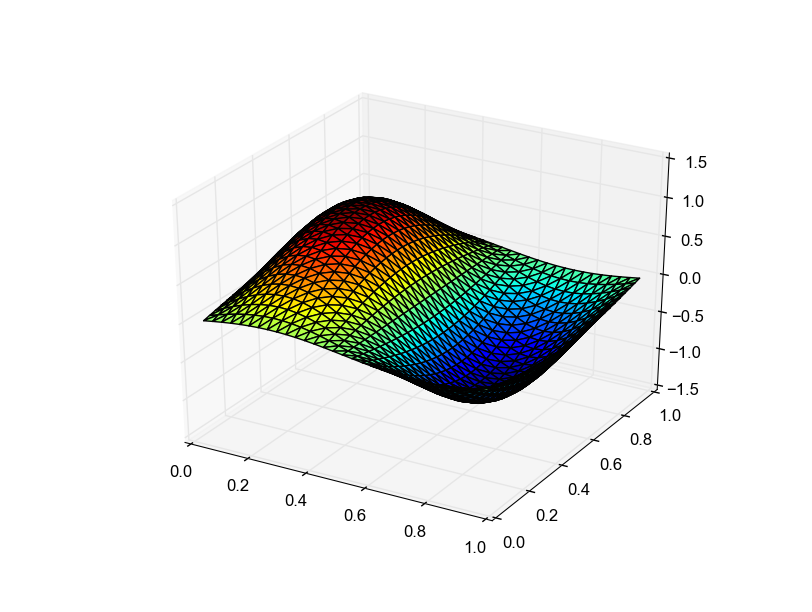
\includegraphics[width=\textwidth, trim={2.5cm 1.25cm 2.5cm 2cm}, clip]{./Figures/surfplot_key2_5.png}
  \end{subfigure}%
  \quad
  \begin{subfigure}[b]{0.48\textwidth}
    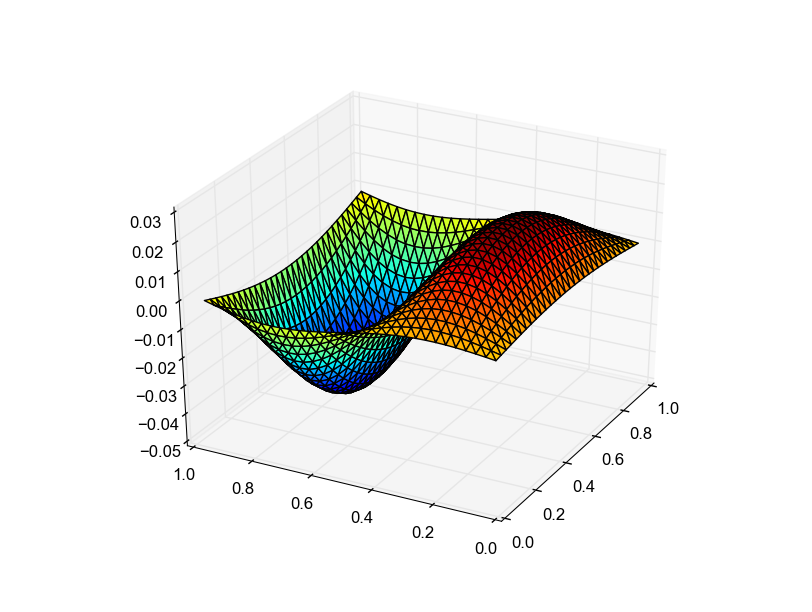
\includegraphics[width=\textwidth, trim={2.5cm 1.25cm 2.5cm 2cm}, clip]{./Figures/surfplot_key3_5.png}
  \end{subfigure}
  \quad
  \begin{subfigure}[b]{0.48\textwidth}
    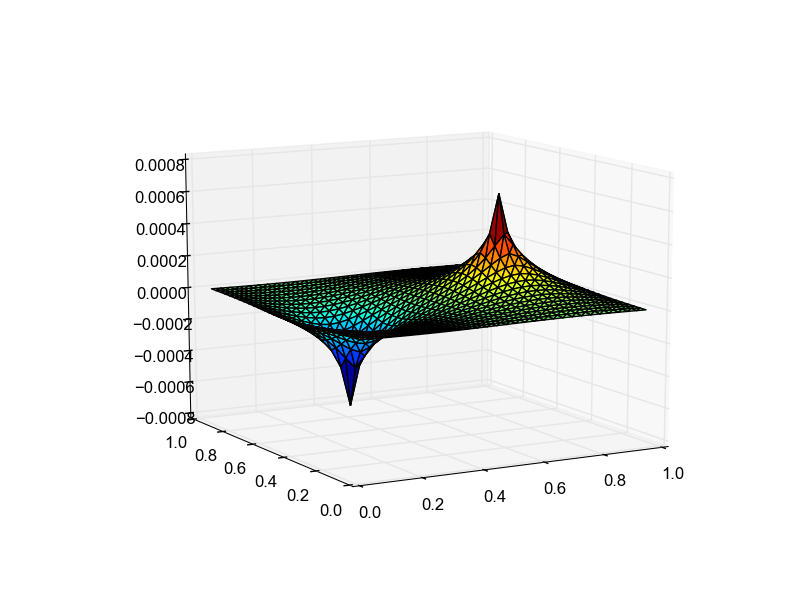
\includegraphics[width=\textwidth, trim={2.5cm 2cm 2.5cm 2cm}, clip]{./Figures/surfplot_key4_5.png}
  \end{subfigure}
          %(or a blank line to force the subfigure onto a new line)
  \vspace{1\baselineskip}
  \caption{The obtained solutions to Poisson's equation using different source functions. The upper left, 
     right and lower subfigure show the solutions for
     %$f(x,y) = \sin ( 2 \! \pi \! x ) \sin ( \pi \! y )$,
     $f(x,y) = 5 \pi^2 \sin (\pi \! x ) \sin (2 \! \pi \! y )$,
     $f(x,y) = e^x \sin ( 2 \! \pi \! x )\sin ( \pi \! y )$ and a 
     sink-source-function, respectively. 
     }
  \label{fig:f}
\end{figure}
%
